%%%%%%%%%%%%%%%%%%%%%%%%%%%%%%%%%%%%%%%%%%%%%%%%%%
% This template was created by Sean Peneyra.  Share freely.
%%%%%%%%%%%%%%%%%%%%%%%%%%%%%%%%%%%%%%%%%%%%%%%%%%

%      Some common commands using the packages below. 
%      Copy and paste the code below the description. Then remove the percentage signs:

%     Description: Add an image (make sure your image file is in the same folder as this tex file
%\begin{figure}[htbp]
%\scalebox{.4}{\includegraphics{image.jpg}}
%\caption{Add a caption here}
%\end{figure}

%     Description: Add a code file.  Useful for correctly formatting external files
%\lstinputlisting[language=Matlab]{code.m}

\documentclass[letterpaper,notitlepage]{article}
\usepackage[top=1.4in, bottom=1.4in, left=1.35in, right=1.35in]{geometry}
\usepackage[english]{babel}
\usepackage[utf8]{inputenc}
\usepackage{amssymb}
\usepackage{amsmath}
\usepackage{amsthm}
\usepackage{array}
\usepackage{listings}
\usepackage{color}
\usepackage{xcolor}
\usepackage{graphicx}
\usepackage{fancyhdr}
\usepackage{mathrsfs}
\usepackage{tikz}
\usepackage{float}
\definecolor{mygreen}{rgb}{0,0.6,0}
\definecolor{mygray}{rgb}{0.5,0.5,0.5}
\definecolor{mymauve}{rgb}{0.58,0,0.82}
\lstset{language=C,backgroundcolor=\color{white},basicstyle=\footnotesize,breakatwhitespace=false,breaklines=true,captionpos=b,commentstyle=\color{mygreen}, keywordstyle=\color{blue},numbers=left,numbersep=5pt,numberstyle=\tiny\color{mygray},rulecolor=\color{black},stringstyle=\color{mymauve},tabsize=2,title=\lstname}
\pagestyle{fancy}
\fancyhf{}

%%%%%%%%%%%%%%%%%%%%%%%%%%%%%%%%%%%%%%%%%%%%%%%%%%
% Change rhead to name, Change lhead to Homework # or Title
\rhead{Sean Peneyra}

\rfoot{\thepage}
\begin{document}

%%%%%%%%%%%%%%%%%%%%%%%%%%%%%%%%%%%%%%%%%%%%%%%%%%
% Change title to Class name. \\ indicates a line break.  Use the \Large{} to add subtitle
\title{Advanced Radio-Graphical Undersea System (ARGUS) Documentation}

%%%%%%%%%%%%%%%%%%%%%%%%%%%%%%%%%%%%%%%%%%%%%%%%%%
% Change author and date accordingly
\author{Sean Peneyra}
\date{21 January 2025}

\maketitle
\newcommand{\multideg}[1]{\text{multideg}(#1)}
\newcommand{\LT}[1]{\small{\textsc{LT}(#1)}}
\newcommand{\LM}[1]{\small{\textsc{LM}(#1)}}
\newcommand{\LC}[1]{\small{\textsc{LC}(#1)}}
\newcommand{\posint}[0]{\mathbb Z^n_{\geq 0}}
\newcommand{\lex}[0]{>_{lex}}
\newcommand{\grlex}[0]{>_{grlex}}
\newcommand{\grevlex}[0]{>_{grevlex}}
\newcommand{\braket}[4]{\langle #1\:#2|#3\:#4\rangle}
\newcommand{\Shat}[1]{\hat{S}_{#1}}
\newcommand{\twovec}[2]{\left[\!\begin{array}{c}#1\\#2\end{array}\!\right]}
\newcommand{\twoform}[2]{\left[\begin{array}{cc}#1&#2\end{array}\right]}
\newcommand{\threevec}[3]{\left[\begin{array}{c}#1\\#2\\#3\end{array}\right]}
\newcommand{\threeform}[3]{\left[\begin{array}{ccc}#1&#2&#3\end{array}\right]}
\newcommand{\twomatrix}[4]{\left[\begin{array}{cc}#1&#2\\#3&#4\end{array}\right]}
\newcommand{\oc}[0]{\twomatrix{1}{0}{0}{1}}
\newcommand{\ic}[0]{\twomatrix{i}{0}{0}{-i}}
\newcommand{\jc}[0]{\twomatrix{0}{1}{-1}{0}}
\newcommand{\kc}[0]{\twomatrix{0}{i}{i}{0}}
\newcommand{\ob}[0]{\mathbf{1}}
\newcommand{\ib}[0]{\mathbf{i}}
\newcommand{\jb}[0]{\mathbf{j}}
\newcommand{\kb}[0]{\mathbf{k}}
\newcommand{\threematrix}[9]{\left[\begin{array}{ccc}#1&#2&#3\\#4&#5&#6\\#7&#8&#9\end{array}\right]}
\newcommand{\ma}[1]{\measuredangle #1}
\newcommand{\Amatri}[0]{\threematrix{e^t}{2e^{-t}}{e^{2t}}{-e^t}{2e^{-t}}{e^{2t}}{3e^t}{-e^{-t}}{-e^{2t}}}
\newcommand{\Bmatri}[0]{\threematrix{2e^t}{e^{-t}}{3e^{2t}}{2e^t}{e^{-t}}{-e^{2t}}{-e^t}{3e^{-t}}{2e^{2t}}}
\newcommand{\del}[0]{\partial}
\newcommand{\delx}[1]{\frac{\partial #1}{\partial x}}
\newcommand{\dely}[1]{\frac{\partial #1}{\partial y}}
\newcommand{\bey}[0]{\begin{equation}}
\newcommand{\eey}[0]{\end{equation}}
\newcommand{\ben}[0]{\begin{equation}}
\newcommand{\een}[0]{\end{equation}}
\newcommand{\bay}[0]{\begin{align}}
\newcommand{\eay}[0]{\end{align}}
\newcommand{\ban}[0]{\begin{align}}
\newcommand{\ean}[0]{\end{align}}
\newtheorem*{addnote}{Note}
\newtheorem*{addwarn}{Warning}
\newtheorem*{addsoln}{Solution}
\setcounter{section}{0}

%%%%%%%%%%%%%%%%%%%%%%%%%%%%%%%%%%%%%%%%%%%%%%%%%%
% Your paper starts here. Put a blurb before you start the first \section if you like
This program is designed to compress a weather image into as small a text file as possible without sacrificing accuracy.  It was designed by Aevix (aka Sean Peneyra, former submarine officer).

\section{Procedures.}
\subsection{For the Boats}
If you are on a boat, you can use the following general procedure:

\subsubsection{While in active communications}
\begin{enumerate}
    \item Download the most recent version of ARGUS.exe as well as the most recent Template folder.  At the time of the program creation, these files were provided by JHU reps in port.
    \item Put those files onto an approved system.  At the time of this program creation, only the JHU stand-alone laptop was approved for use with the program.  In the future, I hope this program is made available on CANES and NMCI computers.
\end{enumerate}

\subsubsection{While in Emmisions Control (EMCON)}
\begin{enumerate}
    \item Recieve a weather gif message on VLF
    \begin{addnote} This will be a message which contains the characters ``A1R1G2U3S5'' and whos body is promarily non-human readable gibberish made up of A-Z, a-z, and 0-9 characters.\end{addnote}
    \item Put the entire message into a text file (.txt) and transfer the file to the information system which can run the ARGUS.exe program
    \begin{addnote} If that system is the JHU standalone laptop, this will entail burning a CD in radio and loading the message file onto the standalone laptop.  If the information system is CANES, there will be no need to burn a CD, but you will have to save the message as a .txt somewhere. \end{addnote}
    \item Open the ARGUS.exe program $\rightarrow$ It will open a file browser
    \item Navigate to the .txt file containing the VLF message and double click the .txt file
    \item Your image should open $\rightarrow$ the image will also be saved in the same folder as the .txt file.
\end{enumerate}

\subsubsection{Troubleshooting}
If you get an error, the problem may be one of the following.
\begin{enumerate}
    \item you do not have the most recent template folder from the BCA.  
    \begin{addsoln} The template used to create the message shoreside must be the same as the template onboard the boat for the image to compile correctly. Go download the new set of templates once out of EMCON.\end{addsoln}
    \item you are trying to open the file directly from a portable media storage device (aka the CD you used to pull the message from radio) 
    \begin{addsoln} The program tries to save the image output in the same folder as the .txt file. If your .txt file is on a CD, it will struggle to add data to the CD, then give up. Save the message to a local folder.\end{addsoln}
    \item you do not have the most recent ARGUS program  
    \begin{addsoln} I am actively working to make the program: more accurate, better at compression (smaller VLF messages), smoother functioning, more user friendly, more efficent, and faster running.  Please excuse the active construction. Go obtain the most recent program.  Instructions for shoreside on how to get it to the boats is below.\end{addsoln}
    \item the VLF message was garbled
    \begin{addsoln} This program uses complex mathematics (literally) to maximize compression of the information. If any of the characters are missing or substituted, the program will fail to rebuild the image. Pull a clean copy of the message.\end{addsoln}
\end{enumerate}


\subsection{For Shoreside}

\subsubsection{Before you start}
\begin{enumerate}
    \item Ensure you have the latest version of ARGUS.
    \item Ensure the folder which contains the file ``ARGUS.exe'' contains:
    \begin{itemize}
        \item ARGUS.exe
        \item ARGUS.pdf
        \item README.md
        \item Message Template.txt (more details on how to use the message template below)
        \item a folder called templates (may not be there and that is okay)
        \item ----- and no others -----
    \end{itemize}
\end{enumerate}

\subsubsection{Creating a message for the units}
\begin{enumerate}
    \item verify initial conditions from ``BEFORE YOU START''
    \item obtain a weather graphic from METOC
    \item open ARGUS.exe $\rightarrow$ it will open a file explorer
    \item use the file explorer from ARGUS.exe to open the weather gif.
    \begin{addnote} Acceptable file types are .gif and .jpg \end{addnote}
    \item select the correct template from the drop-down (if there is no correct template, follow instructions for CREATING A TEMPLATE below)
    \item enter the DTG for which the graphic is valid
    \item click ``Select Template''
    \item ARGUS will save a message which you will send to the units when there is space available on the applicable VLF broadcast $\rightarrow$ it will also try and open the .txt file for viewing
\end{enumerate}

\subsubsection{Create a new template (simple)}
\begin{addwarn}
    Warning: The boats will not be able to use a new template until they download the template while out of EMCON. I reccomend using existing templates whenever possible.
\end{addwarn}
\begin{enumerate}
    \item follow steps 1-4 from CREATING A MESSAGE FOR THE UNITS
    \item click ``New Template''
    \item follow the on-screen instructions $\rightarrow$ pictures and descriptions below
    \item ARGUS will create a templates folder (if not already there) and create a template for the selected .gif in the templates folder
    \begin{addnote} There should be two files in each folder in templates: a .gif where all the colors are a solid red and a .config file \end{addnote}
    \item ARGUS will save a message which should be sent to the units as space allows on the broadcast $\rightarrow$ it will also try and open this file for viewing
    \item navigate to the folder which contains ARGUS.exe and the templates folder which contains the new template
    \item right click the folder containing all the files and folders listed in BEFORE YOU START
    \item hover over ``compress to'' and click ``.zip'' (for windows 11) - or - hover over ``send to'' and click ``compressed (zipped) folder'' (for earlier versions of windows)
    \item send the zipped file to the boats somehow (either post on a public CFFO website or send to the boats on a disc)
\end{enumerate}


\newpage
\subsubsection{Create a new template (with pictures)}
\begin{figure}[H]
\centering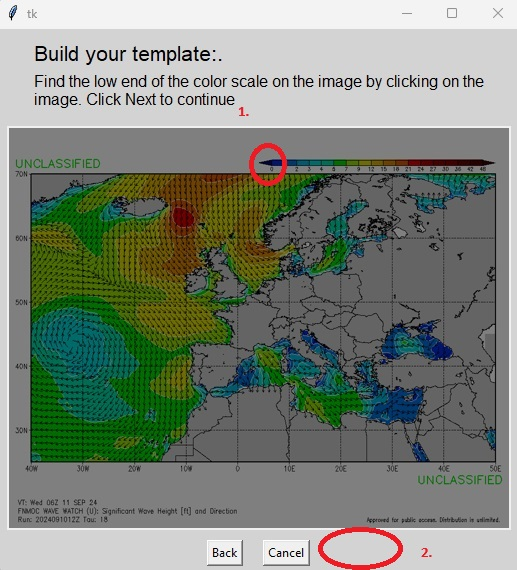
\includegraphics[width=0.5\textwidth]{TeX/Build_Template1.jpg}
\caption{First window displayed to build your own template.}
\end{figure}
This is the first window you will see when starting to build a new template.
\begin{enumerate}
    \item Begin by clicking on the low end of the scale.  This should highlight a small square around where you clicked.  If you click multiple times inside the picture, it will save the last position clicked at.  Ensure everything including the very tip of the scale is highlighted.
    \item There is no ``Next'' button until you click at least once in the picture.  Once you click, ``Next'' will appear.
\end{enumerate}

\newpage
\begin{figure}[H]
    \centering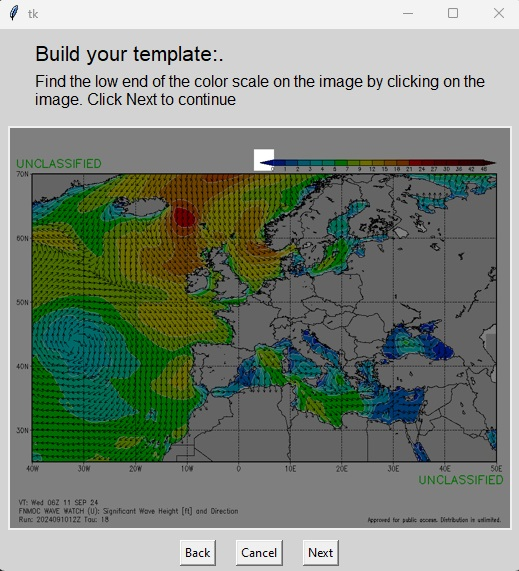
\includegraphics[width=0.5\textwidth]{TeX/Build_Template2.jpg}
    \caption{View after you click at least once inside the picture.}
\end{figure}
Notice how the highlighted box ecompasses all the way to the end of the scale. It will also be important on the next step to ensure the numbers associated with the scale are completely highlighted.  Once you are satisfied with where the highlighted box is, click ``Next''.

\newpage
\begin{figure}[H]
    \centering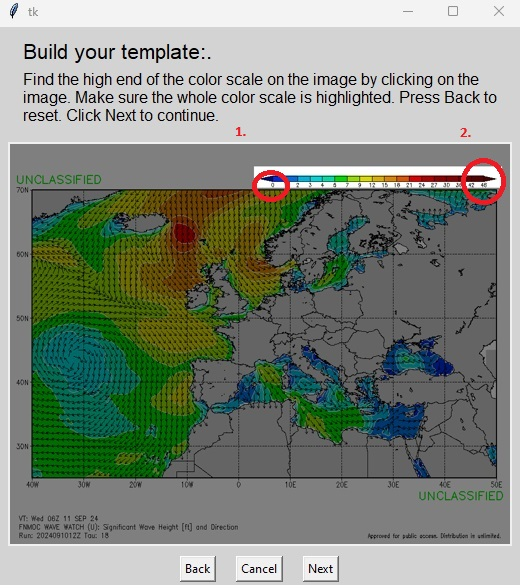
\includegraphics[width=0.5\textwidth]{TeX/Build_Template3.jpg}
    \caption{View after clicking a second time in the picture.}
\end{figure}
After you clicked ``Next'' on the previous step, click back into the picture on the high end of the color scale. You may click as many times as you like to adjust the highlighted box and line it up with the color scale. When you click at least once inside the picture, ``Next'' will appear. When you  are satisfied with where the highlighted box is, click ``Next''.
\begin{enumerate}
    \item Ensure all the numbers associated with the scale are highlighted.
    \item Ensure that both ends of the scale are visible. This highlighted box will be retained in the template and will be produced for the boats when they compile the image on their end.
\end{enumerate}

\newpage
\begin{figure}[H]
    \centering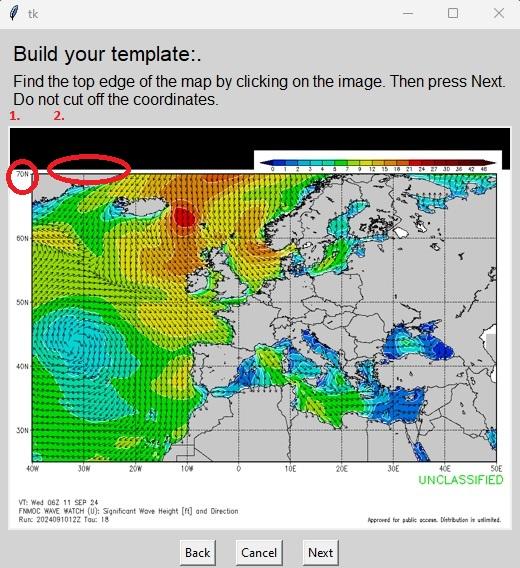
\includegraphics[width=0.5\textwidth]{TeX/Build_Template4.jpg}
    \caption{View after clicking above the top edge of the map.}
\end{figure}
After you clicked ``Next'' on the previous step, click back into the picture above the top edge of the map. You may click as many times as you like to adjust the cropped out area. When you click at least once inside the picture, ``Next'' will appear. When you  are satisfied with where the cropped area appears, click ``Next''.
\begin{enumerate}
    \item Ensure the whole latitude and longitude numbers remain visible.  This will ensure the lat/lon are retained in the template and will be produced for the boats when they compile the image on their end.
    \item Ensure the classification marking is cropped out. If it is left in, the program will interpret the colored letters as wave heights and it will throw off the algorithm. Example shown below.
\end{enumerate}

\newpage
\begin{figure}[H]
    \centering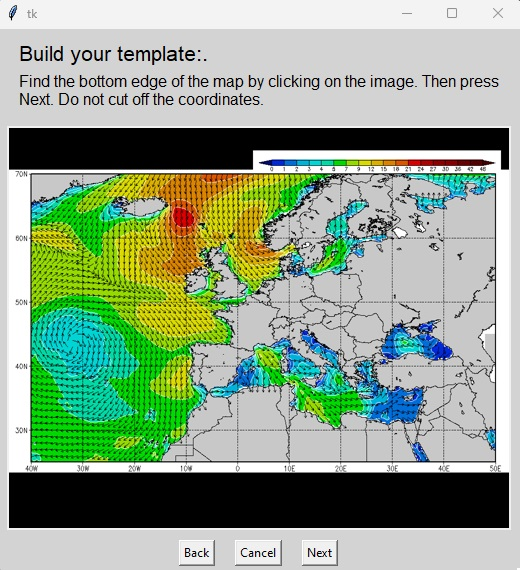
\includegraphics[width=0.5\textwidth]{TeX/Build_Template5.jpg}
    \caption{View after clicking below the bottom edge of the map.}
\end{figure}
After you clicked ``Next'' on the previous step, click back into the picture below the bottom edge of the map. You may click as many times as you like to adjust the cropped out area. When you click at least once inside the picture, ``Next'' will appear. When you  are satisfied with where the cropped area appears, click ``Next''.

\newpage
\begin{figure}[H]
    \centering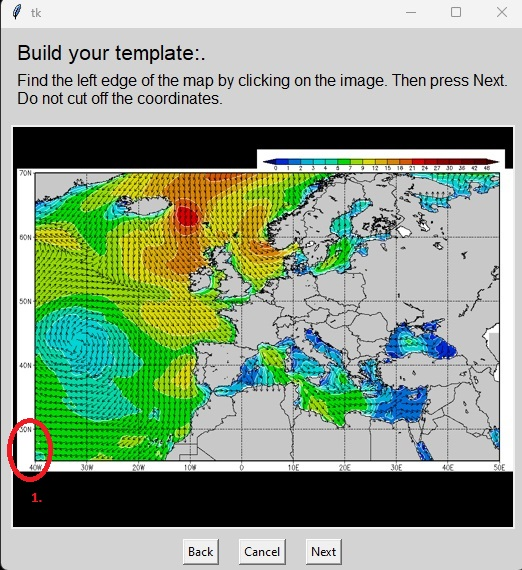
\includegraphics[width=0.5\textwidth]{TeX/Build_Template6.jpg}
    \caption{View after clicking left of the left edge of the map.}
\end{figure}
After you clicked ``Next'' on the previous step, click back into the picture left of the left edge of the map. You may click as many times as you like to adjust the cropped out area. When you click at least once inside the picture, ``Next'' will appear. When you  are satisfied with where the cropped area appears, click ``Next''.
\begin{enumerate}
    \item Ensure the whole latitude and longitude numbers remain visible.  This will ensure the lat/lon are retained in the template and will be produced for the boats when they compile the image on their end.
\end{enumerate}

\newpage
\begin{figure}[H]
    \centering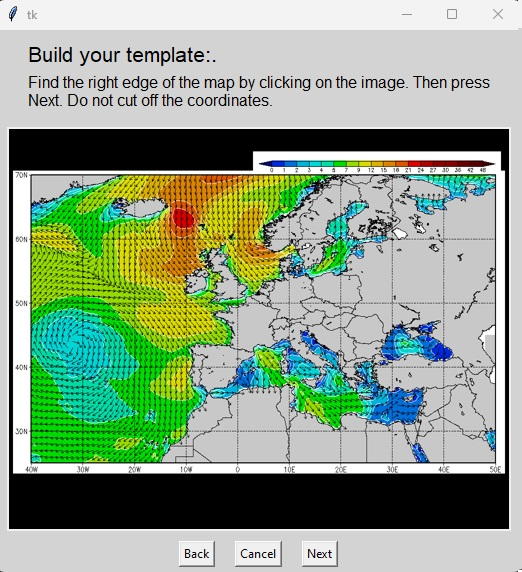
\includegraphics[width=0.5\textwidth]{TeX/Build_Template7.jpg}
    \caption{View after clicking to the right of the right edge of the map.}
\end{figure}
After you clicked ``Next'' on the previous step, click back into the picture to the right of the right edge of the map. You may click as many times as you like to adjust the cropped out area. When you click at least once inside the picture, ``Next'' will appear. When you  are satisfied with where the cropped area appears, click ``Next''. Once you get past this point, there is no back button.  You will have to click ``Cancel'' and start over.

\newpage
\begin{figure}[H]
    \centering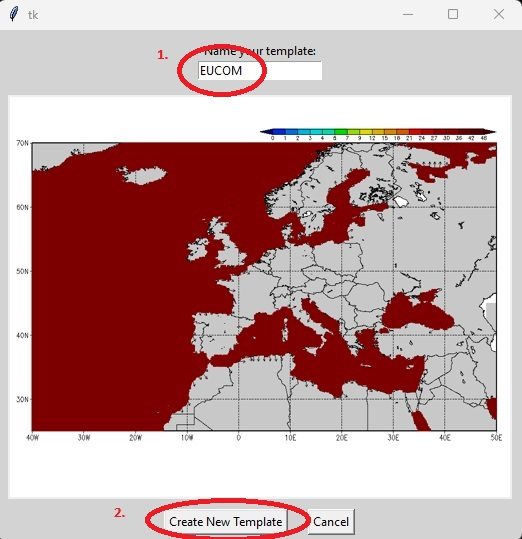
\includegraphics[width=0.5\textwidth]{TeX/Build_Template8.jpg}
    \caption{Final template view.}
\end{figure}
After you clicked ``Next'' on the previous step, name the template. After you click ``Create New Template'' you will be taken back to the template selection screen which should have the new template listed in the drop-down menu.
\begin{enumerate}
    \item You should use the FNMOC naming convention (e.g. ``EPAC'') for the different AORs. This will make it easier for the boats when they rebuild the image.
    \item Once you click ``Create New Template'', a folder will be added to the templates folder with two files inside.  One will be the image of the template saved as a jpg.  The other will be a config file which will help the program rebuild the map from a navy message.
\end{enumerate}


\newpage
\begin{figure}[H]
    \centering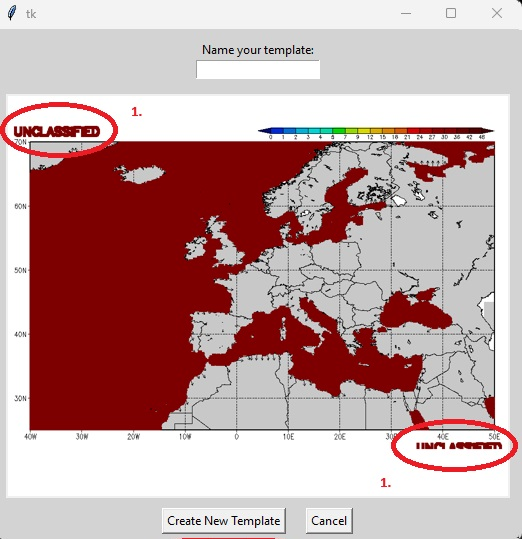
\includegraphics[width=0.5\textwidth]{TeX/Build_Template9.jpg}
    \caption{This is what wrong looks like.}
\end{figure}
As you can see, the user did not appropriately crop out the classification markings.  It interpreted the green text as a waveheight 5-7 foot area. If this happens, fear not. You just need to start over.
\begin{enumerate}
    \item The template contains areas which were originally the classification markings.
\end{enumerate}

\subsection{Using the message template}
In the folder which contains ARGUS.exe, there should be a .txt file named ``Message Template.txt''.  If it isn't there for some reason, feel free to save a .txt file with that identical name. The only rules for the message template are:
\begin{enumerate}
    \item It must contain the line ``\textless message\textgreater '' (exactly those characters, without quotes, and on its own line).  This lets the program know where to put the useful information for the image.
    \item Do not use the characters ``A1R1G2U3S5'' in that order anywhere in the text of the message template.  Those characters indicate to my program where in the final message the useful information for the image starts.
\end{enumerate}

\begin{addnote} Below is what I have loaded as a template by default. Feel free to edit it and save as your own template keeping in mind the rules above:\end{addnote}
\begin{lstlisting}[numbers=none,rulecolor=\color{black}]
R XXXXXXZ MMM YY
FM COMSUBPAC PEARL HARBOR HI
TO SSBN PAC
BT
UNCLAS
SUBJ/VLF WEATHER GIF//
RMKS/SEE INSTRUCTIONS ON CSP WEBSITE ON HOW TO USE THIS MESSAGE.
<message>
BT
#0001
NNNN
\end{lstlisting}

\section{General Notes.}
 The goal for this progam is to:
 \begin{enumerate}
    \item Read an input file
    \item If the input file is an image:
    \begin{enumerate}
        \item Open a GUI to either build or select an existing template
        \item Simplify the image into an array of scalars based on a legend
        \item Build a DFT off of the scalar array
        \item Truncate the DFT
        \item Produce a naval message on compressed list of coefficients
    \end{enumerate}
    \item If the file is a text file:
    \begin{enumerate}
        \item Rebuild the DFT from the naval message
        \item Perform an IDFT to reproduce a scalar array
        \item Interpret build the scalar array into the original input image
        \item Overlay a standard image template over the top of the scalar array
    \end{enumerate}
\end{enumerate}

     Feel free to reach out with any comments or questions.
     Sean Peneyra
     peneyra.s@gmail.com

%%%%%%%%%%%%%%%%%%%%%%%%%%%%%%%%%%%%%%%%%%%%%%%%%%
% bibliography starts here.  update the number of bibitems after (thebibliography)
% \newpage
% \begin{thebibliography}{1}
% \bibitem{Book1}
% Book information
% \end{thebibliography}
\end{document}
